\documentclass[10pt,titlepage]{article}
\usepackage{listings}
\usepackage{color}
\usepackage{graphicx}
\usepackage{subcaption}

\definecolor{mygreen}{rgb}{0,0.6,0}
\definecolor{mygray}{rgb}{0.5,0.5,0.5}
\definecolor{mymauve}{rgb}{0.58,0,0.82}

\lstset{ %
  backgroundcolor=\color{white},   % choose the background color; you must add \usepackage{color} or \usepackage{xcolor}
  basicstyle=\footnotesize,        % the size of the fonts that are used for the code
  breakatwhitespace=false,         % sets if automatic breaks should only happen at whitespace
  breaklines=true,                 % sets automatic line breaking
  captionpos=b,                    % sets the caption-position to bottom
  commentstyle=\color{mygreen},    % comment style
  escapeinside={\%*}{*)},          % if you want to add LaTeX within your code
  extendedchars=true,              % lets you use non-ASCII characters; for 8-bits encodings only, does not work with UTF-8
  frame=single,                    % adds a frame around the code
  keepspaces=true,                 % keeps spaces in text, useful for keeping indentation of code (possibly needs columns=flexible)
  keywordstyle=\color{blue},       % keyword style
  language=Octave,                 % the language of the code
  numbers=left,                    % where to put the line-numbers; possible values are (none, left, right)
  numbersep=5pt,                   % how far the line-numbers are from the code
  numberstyle=\tiny\color{mygray}, % the style that is used for the line-numbers
  rulecolor=\color{black},         % if not set, the frame-color may be changed on line-breaks within not-black text (e.g. comments (green here))
  showspaces=false,                % show spaces everywhere adding particular underscores; it overrides 'showstringspaces'
  showstringspaces=false,          % underline spaces within strings only
  showtabs=false,                  % show tabs within strings adding particular underscores
  stepnumber=2,                    % the step between two line-numbers. If it's 1, each line will be numbered
  stringstyle=\color{mymauve},     % string literal style
  tabsize=2,                       % sets default tabsize to 2 spaces
  %title=\lstname                   % show the filename of files included with \lstinputlisting; also try caption instead of title
}

\begin{document}
  \title{LED Chandelier}
  \author{Toan Vuong and Sam Mansfield\\
          Mentor: Mark Oehlberg
          EECS149\\
         }
  \date{December 19th, 2013}
  \maketitle

  \section*{Introductions}
    Inspired by a UPENN interactive cube, our group set out to create an array of interactive LED chains that together, would form a chandelier. To do this, we outlined three goals to be accomplished:
    \begin{enumerate}
    \item Scalability--We want our project to be scalable and expandable. The possibility of seamlessly integrating more and more strands.
    \item Low cost--The cost of each strand must be low. Since the idea is to have many strands, the cost of each strand, when scaled to a large quantity, is significant.
    \item Low power--Each strand will be self-powered. As such, they would need to use power efficiently and keep their power usage low to minimize the size of onboard power supplies.
    \end{enumerate}

    Though the end result is to simulate a low-resolution 3D-display, we were also interested in identifying a concept for expanding such a display if need be. Thus born the idea of individually-acting strands. Each strand would have all the components it would need to reflect the environment underneath. Together, a square array of strands would reflect a certain region overwhich they all enclose. Because no strands know about any other strands, we could easily add more strands to create a larger and more immersive display.

  \section*{Approach}
  The interactive cube, from which our project derives, is popular among the LED hobbyists and embedded programmers. Cubes tend to be of varying sizes, from 3x3, to 4x4, to 8x8, and even 16x16. From simple single-colored LEDs to RGB LEDs, they exist all over the net.\\ 

  In fact, our initial approach was to make a 3x3 cube. Using a Teensy 2.0, 9 LEDs, an ultrasonic sensor, some resistors and basic soldering skills, we created our first prototype cube. It worked well, but was too simplistic and uninteresting. We wanted something a bit different from the rest. \\

  That is why together with our mentor, we decided to create a more unique LED matrix: a chandelier. We knew from the start that our project will require a long time overhead to complete since many of the parts will need to be ordered en masse. The parts would have to be picked out carefully. Since our budget was only \$200, we had to use any parts that ESG could provide and have on hand. Luckily, they had plenty of MSP430 microprocessors, and so we decided to use those as the brains for our LED strands. Lucky for us, these were extremely low-powered, and uses low voltages in the range of 1.8-3.6V. \\

  We looked into several types of LEDs, and rejected many. Pre-built strands of LEDs exist, but none did what we wanted, and most were too expensive to get a large quantity of. Some weren't individually addressable; others were partly covered up due to the way they were built. In the end, creating our own strands was the best option. \\

  Our requirements were simple: To create a strand that would emphasize the LEDs, and nothing else. To achieve this, we needed to minimize the profile of our wires. This meant that we needed to choose extremely thin wires. In particular, we went with 36AWG magnet wires. To support our strands of LEDs, we put them inside clear heatshrink tubing. \\

  Next up was choosing an appropriate sensor to measure the environment underneath. Though initially we considered a single sensor range finder for its small profile, we found that it was too expensive to get in large quantities. Furthermore, ESG had many of the standard, dual sensor range finders (SRF05) in stock. Thus, we went with those. \\ 
  \begin{figure}[h!]
      \centering
      \begin{subfigure}[b]{0.48\textwidth}
      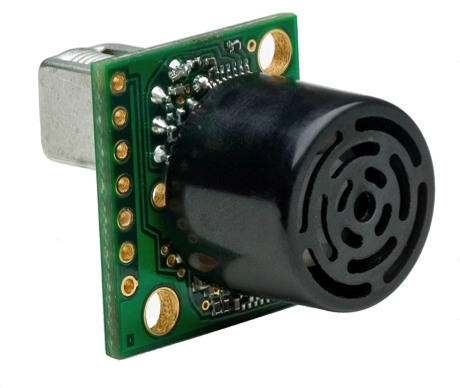
\includegraphics[width=\textwidth]{max.png}
      \caption{A single sensor ultrasonic range finder}
      \end{subfigure}
      \begin{subfigure}[b]{0.48\textwidth}
      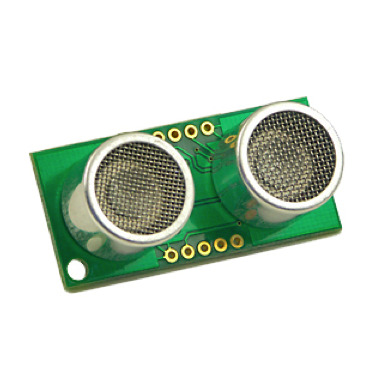
\includegraphics[width=\textwidth]{srf05.png}
      \caption{SRF05. Dual sensor range finder}
      \end{subfigure}
      \caption{Two different range finders}
  \end{figure} 

  Using the parts we chose, we created our strand prototype: A working, single strand of 8-bit LEDs representing one pixel with 8-bits of depth resolution. We then began to familiarize ourselves with programming the hardwares: In particular the MSP430 and the ultrasonic sensor. With the basic hardware and software in place, we got around to ordering the rest of our parts, enough to create 16 strands. We also created an Eangle layout of our circuitry in order to reduce its footprint, with the intention of further concealing everything that wasn't LEDs from the viewer's eyes. \\

  \section*{Models and Algorithms}
  Our program continuously reads from the range finder, updating the LEDs as the readings changes. More formally, we modeled it as a simple state machine as in Figure 2. \\
  \begin{figure}[h!]
      \centering
      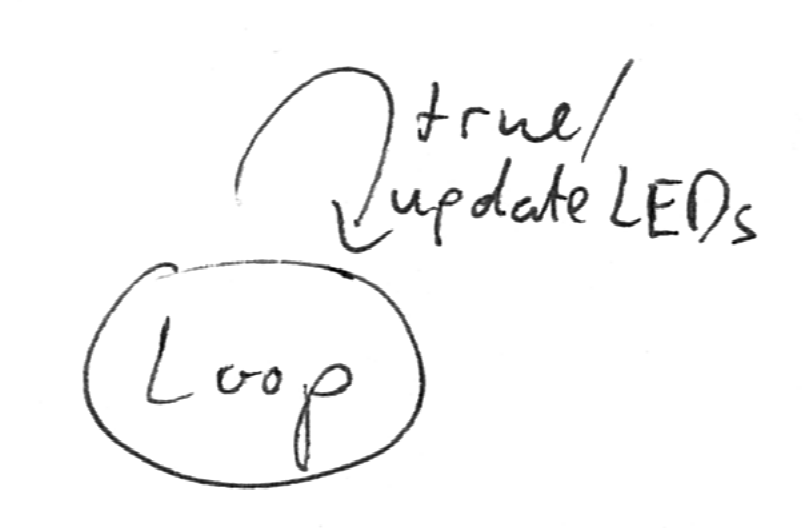
\includegraphics[scale=0.75]{1.png}
      \caption{Main program state machine}
  \end{figure}

  We have a main loop, which turns on the LEDs as appropriate. The exact LEDs to be turned on or off are determined by the last reading of the sensor. The sensor is read on an interrupt, and this value is saved to a variable that the main loop reads. Since each LED is connected to a separate pin, we merely had to turn on or off a memory-mapped register to alter the LED's state. \\

  Our next task is to add further logic to enable multiple modes. To support this, we used hierarchical modeling for each mode. In particular, the overall program consists of subprograms, only one of which would be active at any given time. Each subprogram contains its own state machine, which runs while the main machine is in that particular state. Figure 3. demonstrates the overall state machine as well as each individual state machine, one of which is our initial program, already shown in Figure 2. \\
  \begin{figure}[p]
      \centering
      \begin{subfigure}[b]{0.7\textwidth}
      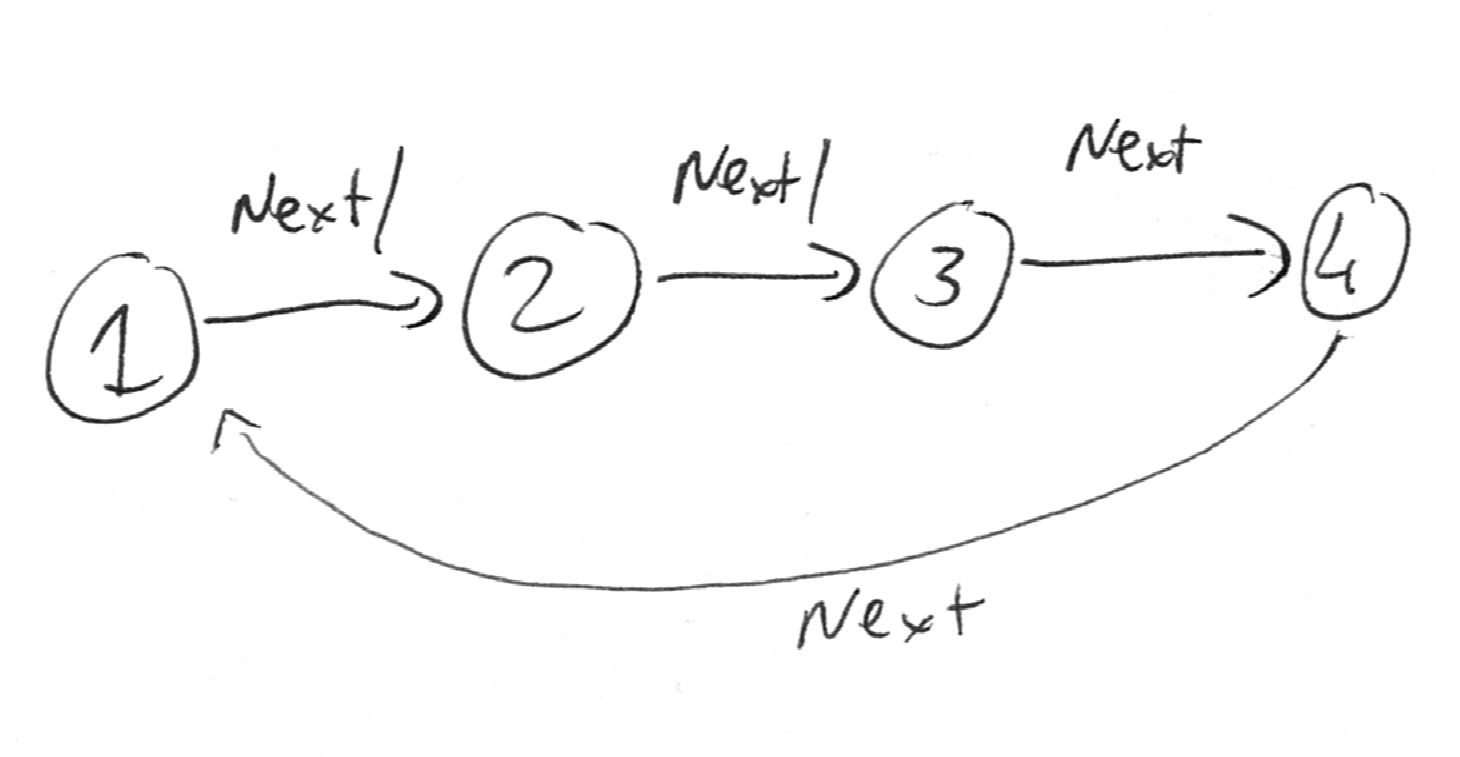
\includegraphics[width=\textwidth]{all.png}
      \caption{Top level state machine}
      \end{subfigure}
      \begin{subfigure}[b]{0.48\textwidth}
      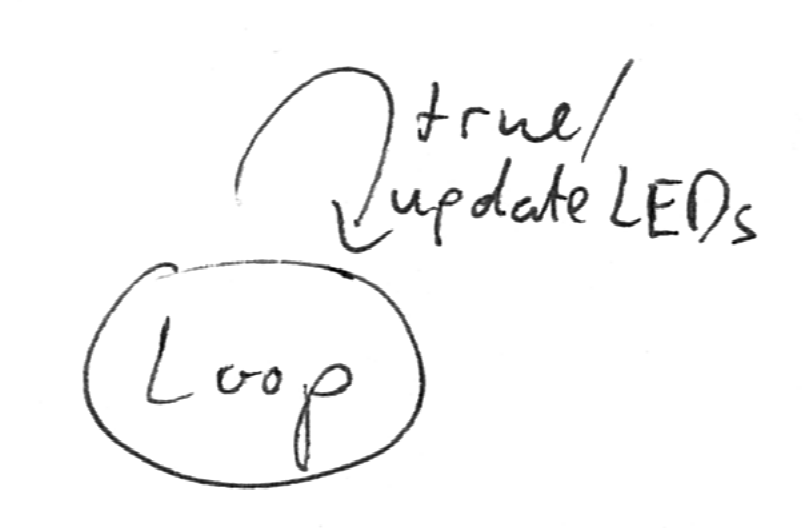
\includegraphics[width=\textwidth]{1.png}
      \caption{Program 1 state machine}
      \end{subfigure}
      \begin{subfigure}[b]{0.48\textwidth}
      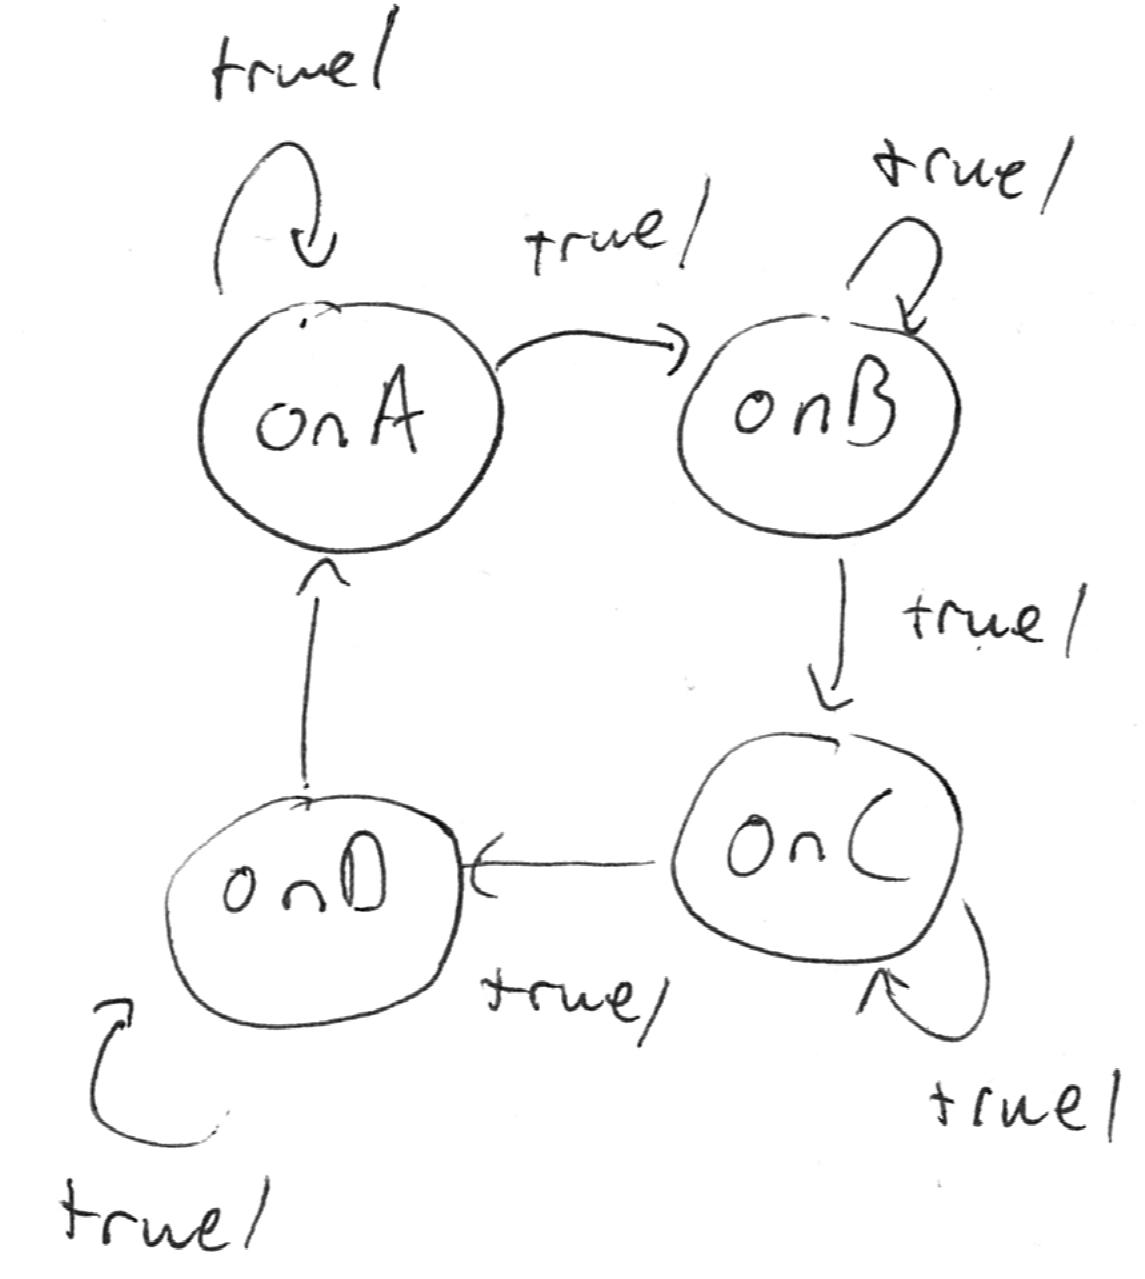
\includegraphics[width=\textwidth]{2.png}
      \caption{Program 2 state machine}
      \end{subfigure}
      \begin{subfigure}[b]{0.48\textwidth}
      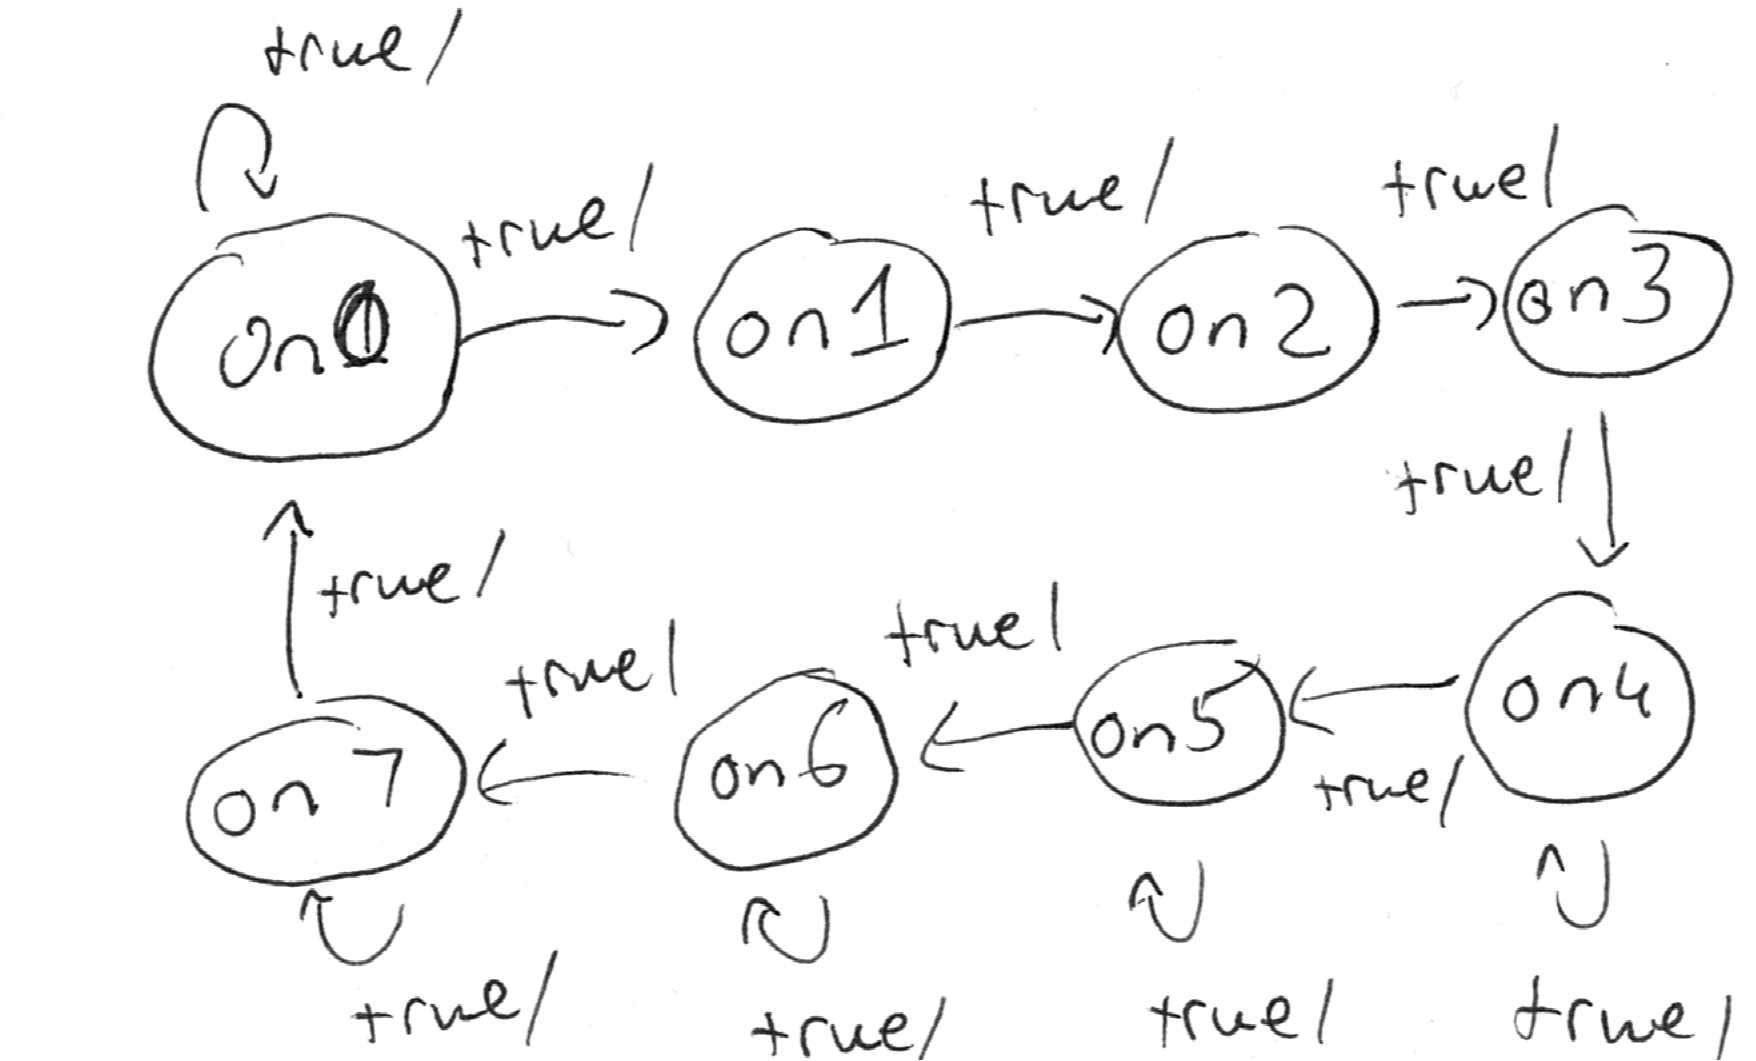
\includegraphics[width=\textwidth]{3.png}
      \caption{Program 3 state machine}
      \end{subfigure}
      \begin{subfigure}[b]{0.48\textwidth}
      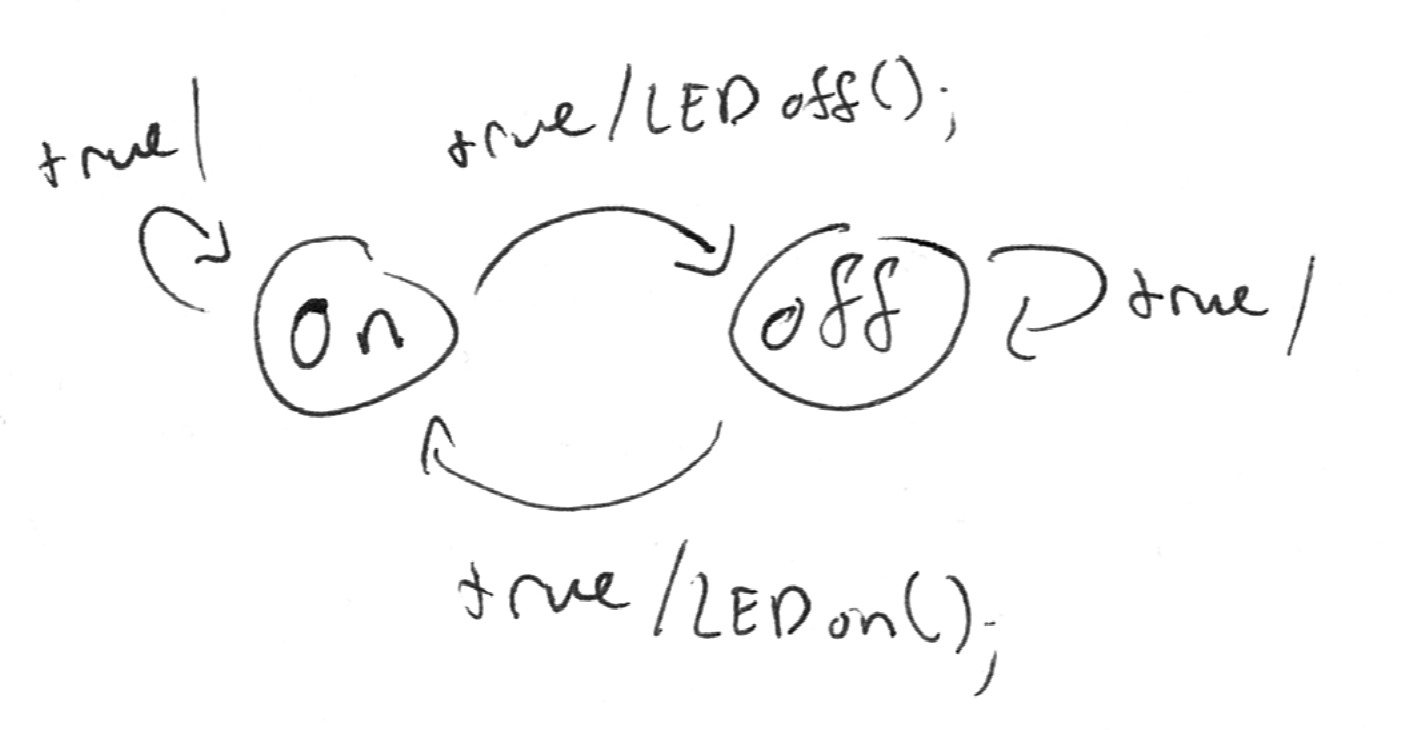
\includegraphics[width=\textwidth]{4.png}
      \caption{Program 4 state machine}
      \end{subfigure}
      \caption{Hierarchy of state machines}
  \end{figure} 

  The idea is that, at any given time, our program will be in one of four modes:
  \begin{enumerate}
      \item[\textbf{Mode 1: }] Object detection, as described above.
      \item[\textbf{Mode 2: }] Pairs of LEDs will turn on, starting with the two outermost, then the two second outermost, etc. In binary:\\
          10000001 \\
          01000010 \\
          00100100 \\
          00011000 \\
          10000001 
      \item[\textbf{Mode 3: }] A single LED will be on at any given time, followed by an adjacent LED, intended to simulate raindrop. In binary from top to bottom:\\
          10000000 \\
          01000000 \\
          00100000 \\
          00010000 \\
          etc.
      \item[\textbf{Mode 4: }] All LEDs will flash with a speed varying depending on the distance detected by the range finder. In binary:\\
          11111111 \\
          00000000 
  \end{enumerate}

  Though our state machine models are non-deterministic (In particular a single state may have multiple active transitions), the program is not. The self-transitions act as a timer, whereas the non-self transition is only ever active when the state's time is up. Thus, for all time, if the non-self transition is active, the machine would take that transition. Otherwise, it remains in the same state. For mode 2 and 3, this time is random. For mode 4, it is exponentially scaled by the distance, with a small amount of randomness. We did not model our programs as a timed automata. However, given appropriate clock functions and a random function, we could have. For our use case, the non-deterministic models were more than sufficient for implementation.\\

  In order to generate random numbers, we used the algorithm outlined in Figure 4. A lack of an OS or even any high-level standard library means that we don't have a built-in random library to call. We used the fact that the value contained in a newly declared variable is unknown and use this as our random number. We then treat this number as an address, and read from it for the next random number. Continuing this process gives us as many random numbers as needed. One potential pitfall is the possibility that an address contains itself as the value. Thus, it would become a fixed-point in our algorithm. To disallow this, we merely declare another integer and read from that in such a case. One other issue that this algorithm may access memory it should not. Though we have not yet encountered such a case, it is not difficult to limit the memory space accessed to a valid memory region, and to retry else where if an address is outside this region.\\
  \begin{figure}[h!]
      \centering
      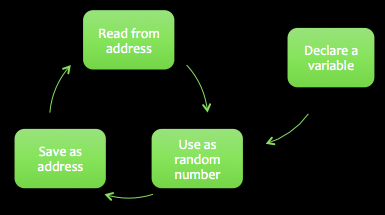
\includegraphics[width=\textwidth]{ran.png}
      \caption{Randomness algorithm}
  \end{figure}

  \section*{Challenges}
  We did not have any extra pins for inputs to change programs. Instead, we relied on the ultrasonic sensor. If it reads value in a certain range for a certain amount of time, then the main state machine would proceed to the next state. Initially, we wanted to use the reset pin as well as the fact that global variables do not reinitialize on reset to keep track of the main state. Unfortunately, the MSP430 does reinitialize all variables upon reset, and thus this was not possible. \\
  
  Assembly was particularly challenging given that we had to put a strand of LEDs held together by thin and fragile wires through a heatshrink tube. We faced many issues, including LEDs burning out within the heatshrink tubes and soldering small surface mount parts. To aid with assembly, we had a laser cut template on which we solder the LED strands before putting them through the heatshrink. To keep our strand footprint small and to minimize the amount of soldering, we designed custom PCB boards on which our circuitry would live. Even with all these aids, each strand takes upwards of three hours to create.\\
  
  In addition to using thin magnet wires and clear heatshrinks, we chose wide angle LEDs for a better viewing from an external point of view. Our PCBs are also designed as small as possible so as to not distract the viewer from the LEDs. \\

  One particular challenge that we were never able to overcome was the interference between ultrasonic sensors. The sensor angles are quite wide, limiting the minimal space between strands to be over one foot lone. This ultimately affects the resolution of our chandelier. To counteract this, we wrapped a fuzzy material around the sensor in hopes that the fuzziness would absorb the ultrasonic sounds (as opposed to merely reflecting them). Unfortunately, this approach did not work. Though the interference readings were initially gone, the material causes erratic behaviors in the sensors, and were ultimately unreliable. \\

  \section*{Summary}
  Overall we accomplished our goal of creating strands for a chandelier. Each strand is individually controlled, and costs are reasonable (About \$16 per strand), which could be driven lower by buying in bulk. Unfortunately the strands are difficult to assemble, adding a large labor overhead. In addition, we would need to solve the interference issue if our chandelier is to represent accurately the environment on which it hangs. \\

  For future work, we intend to investigate pre-built strands of LEDs to remove the assembly overhead. Furthermore, we would like to look into creating our own circuitry for the ultrasonic sensor to drive down the cost as well as the sensor angle. \\

  One major area that should be explorer is the addition of an external camera to replace individual range finders. This would allow for external synchronicity between the strands and also would remove the issue of interference at the cost of scalability (Which can be compensated with additional software logic). However, doing such requires a server and client architecture, wherein the camera becomes a server which provides information to each client strand on which LEDs to light up. Each client strand would also need a wireless radio to communicate to the server. \\

  \section*{Roles}
  Toan primarily contributed to ideas on approaching the project and to further distinguish the project from the standard LED cube projects available, as well as providing inputs for hardwares. He ordered some of the hardware, and architected most of the software, including usage of the sensors and the MSP430 itself. Sam came up with the initial idea for the project, and worked with Mark on creating both the PCB layout and the PCBs themselves. He virtually all of the soldering and assembly, and also gathered parts required. We both worked on each of the milestones and presentation, as well as the final report. \\
  \section*{Key Concepts and Feedback}
  Though it should be obvious from the above, concepts we used include hierarchical state machine modeling, memory hierarchy, interrupts, and the overall designing of our system. Everything that we used were well within the scope of the class. One key area that we could have benefited from is creating (or approximating) algorithms that are normally provided in standard libraries, such as the random number generator. However, this is surely only specific to our project, cannot be generalized, and therefore the class as a whole may not benefit. 

\end{document}
